\chapter{Molecular evolution}
\minitoc
\label{sec:intro}

From the discovery of evolution to today knowledge, the understanding of the mechanisms from which the diversity of life and complexity emerges has seen dramatic changes, and revolution.
Much as been done in comprehension, gathering of empirical data and development of theoretical tools.
This introduction will recall assumptions and limitations on which this work is based.
It will emphasis the milestones and their respective contribution, while doing its best to highlight the undertaken paths which have been forgotten with time.
It is a modest attempt neither exhaustive nor accurate, imprinted with ideology of our current society on how we perceive and interpret past discoveries.
Moreover, this introduction will highlight a few names, while the bulk of the work has been done by unmentioned and sometimes forgotten scientists.

\section{Historical perspective}

Molecular evolution is a recent scientific fields, emerging at the crossroad of evolutionary biology which had seen tremendous theoretical development in the nineteen century, and molecular biology which had seen many technical revolutions.
It borrows strength from both fields, on one hand the amount of empirical data available from molecular biology, and the predictive power of population-genetics.
In molecular evolution, the pattern of sequences distribution in different population and organism inform us both on the past of individuals, population and species, while at the same time shining light on molecular processes generating such distribution.

Population-genetic historically emerged as an unifying theory between 
Mendelian inheritance and quantitative genetic.
The argument mainly revolved around th evolution of characters  discrete 
Soon after the rediscovery of Mendel's laws of inheritance, a fierce debate opposed two groups of biologists: Mendelians who believed that evolution was driven by mutations transmitted by the discrete segregation of alleles \citep{bowler2003evolution}, and biometricians who claimed that variation was continuous.
The first group, led by Bateson and de Vries, maintained that the variations measured by biometricians were too small to account for evolution while the second, led by Karl Pearson (1857--1936) and Walter Weldon (1860--1906), rejected Mendelian genetics on the basis that it would necessarily imply discontinuous evolutionary leaps \citep{provine2001origins}.

It was only fifteen years later that the British statistician Ronald A.\ Fisher (1890--1962) reconciled both theories, first by proving mathematically that mutiple discrete loci could result in a continuous variation \citep{fisher1919xv} and then by showing in subsequent papers and in his book \citep{fisher1930genetical} that natural selection could change allele frequencies in a population and result in evolution.
Soon after, in a series of ten papers named \citep{haldane1927mathematical}, another British geneticist — John B.\ S.\ Haldane (1892--1964) — derived equations of allele frequency change at a single locus under a broad range of conditions.
This allowed him to re-establish natural selection as the major cause of evolution \citep{haldane1932causes}.
The contributions of the two of them, - together with that of Sewall Wright (1889--1988), a geneticist living across the Atlantic who worked out the mathematics for combinations of interacting genes, - laid the foundations for population genetics, a discipline which basically integrated Mendelism, Darwinism and biometry.

The emergence of this new field of study was the first step towards the development of a unified theory of evolution named the ‘modern synthesis’ \citep{huxley1942evolution}. 
Its founders — Theodosius Dobzhansky (1900--1975), George Ledyard Stebbins Jr.\ (1906--2000) and Ernst Mayr (1904--2005) — all defined it on the basis of natural selection acting on the heritable variation supplied by mutations \citep{mayr1959where,stebbins1966processes,dobzhansky1974chance}.
But the exclusive contribution of this adaptive process to genome evolution was soon to be contested.

\subsection{Central dogma of molecular biology}

The discovery of \acrshort{DNA} in the mid-twentieth century \citep{franklin1953molecular,watson1953molecular,wilkins1953molecular} brought about a real revolution in the study of evolution and even led to the establishment of a new research field to which this thesis belongs: molecular evolution — now rather called evolutionary genomics for whole genomes, rather than single genes, get analysed.

From polymerase chain reaction (PCR) to .

\subsection{Neutralists and selectionists}

One of Wright's main contributions to population genetics was the introduction of the concept of ‘adaptive landscapes’ according to which phenomena other than natural selection, — like genetic drift and inbreeding, — could push small populations away from adaptive peaks, thus propelling, in turn, natural selection to drive them towards different adaptive peaks \citep{wright1932roles}.
As such, the relative contributions of neutral forces (like genetic drift) and adaptive forces (like natural selection) became a major subject of debate between Wright and Fisher \citep{plutynski2007drift}.

But this controversy really intensified after Motoo Kimura (1924--1994) proposed the neutral theory of molecular evolution \citep{kimura1968evolutionary,kimura1991neutral,kimura1986dna} and Tomoko Ohta (born 1933) adapted it as the nearly neutral theory \citep{ohta1973slightly}.
For selectionists, most mutations are either beneficial or harmful and are thus either retained or purged by the action of natural selection, whereas supporters of the neutral theory claim that most mutations are adaptively neutral and thus become fixed in populations through the cumulative effect of sampling drift \citep{lewin1996patterns}.

As of today, it is widely accepted that both genetic drift and natural selection participate in the evolution of genomes: the controversy is no longer strictly dichotomous but rather concerns the quantitative contributions of adaptive and of non-adaptive evolutionary processes.

\section{Population-genetics of \acrshort{DNA}}
In this section, we revise the most general cases of models for sequence evolution and their assumptions, their parameters and assumptions.


\subsection*{Single polymorphic site under selection}
The Wright-Fisher model describe the change in frequency of single polymorphic site with two alleles in a population over time. The model makes the following assumptions:
\begin{itemize}
	\setlength\itemsep{-0.2em}
	\item Non-overlapping generations
	\item Constant population size in each generation
	\item Random mating
\end{itemize}

Consider a population of $\Ne$ diploid individuals that has a single polymorphic site with two alleles, one ancestral (fitness = $1$) and one derived (fitness = $1+s$). Assuming no dominance and no recurrent mutation, the probability, $p_{ij}$, that there are $j$ copies of the derived allele present at generation $G+1$ given i copies of the derived allele present at generation $G$ is given by the following binomial calculation:
\begin{align}
	p_{ij} & = \binom{2 \Ne}{j} \left( \dfrac{x(1+s)}{x(1+s) + (1-x)} \right)^j \left(1 - \dfrac{x(1+s)}{x(1+s) + (1-x)} \right)^{2 \Ne -j}, 
\end{align}
where $x = i / 2 \Ne$ is the derived allele frequency in generation $G$.\\

In this discrete framework, it has been shown to be extremely difficult to explicitly derive formulas for several quantities of evolutionary interest. However, as the size of the population approaches infinity (i.e. $ \Ne \rightarrow \infty$), and assuming that the scaled selection pressure ($\Ne s $) remain constant, the discrete Markov process given above can be closely approximated by a continuous-time, continuous-space diffusion process.\\


\subsection*{Probability of fixation}

Under the assumption of no recurrent mutation, the derived allele with initial frequency $p$, goes either extinct ($x=0$) or fixed ($x=1$) after a long time.
It is possible to determine the probability of fixation ($p_{\mathrm{fix}}$), by using the Kolmogorov backward equation.
\begin{equation}
p_{\mathrm{fix}}(p, \scaledselcoef ) = \dfrac{1 - \e^{-\scaledselcoef p }}{1 - \e^{-\scaledselcoef}}\text{, where } \scaledselcoef=4\Ne \selcoef 
\end{equation}
\begin{figure}[thbp]
	\begin{center}
		\includegraphics[width=\textwidth, page=3] {figures.pdf}
	\end{center}
	\caption{Probability of fixation}
\end{figure}

For a mutation, meaning for a derived allele with initial frequency $x = 1 / 2 \Ne$ and the probability of fixation ($p_{\mathrm{fix}}$) if given by:
\begin{align}
	p_{\mathrm{fix}} = \dfrac{1 - \e^{-2 s}}{1 - \e^{-4 \Ne s}} \approx  \dfrac{2 s }{1 - \e^{-4 \Ne s}}
\end{align}
\begin{align}
	p_{\mathrm{ext}} = 1 - p_{\mathrm{fix}} = \dfrac{ \e^{2s(2 \Ne -1) } - 1 }{\e^{4 \Ne s} - 1}
\end{align}

\subsection*{Site frequency spectrum}

$g(x) \der x $ is the expected time for which the population frequency of derived allele is in the range $(x, x+\der x)$ before eventual absorption:
\begin{align}
	g(x) & =  & \dfrac{\left( 1 - \e^{- 2 s }\right) \left( 1 - \e^{-4 \Ne s(1-x)}\right)}{ s (1 - \e^{-4 \Ne s})x(1-x)} \\
	& \approx  & \dfrac{2 \left[ 1 - \e^{-4 \Ne s(1-x)}\right]}{(1 - \e^{-4 \Ne s})x(1-x)}
\end{align}

\begin{figure}[thbp]
	\begin{center}
		\includegraphics[width=\textwidth, page=4] {figures.pdf}
	\end{center}
	\caption{Expected time of derived allele}
\end{figure}

In a sample of size $n$, the expected number of copies of the derived allele is defined as a function of $g(x)$:
\begin{align}
	F(i) & = \int_{0}^{1} g(x) \binom{n}{i} x^{i} (1-x)^{n-i} \der x \\
	& = \int_{0}^{1} \dfrac{2 \left[ 1 - \e^{-4 \Ne s(1-x)}\right]}{(1 - \e^{-4 \Ne s})x(1-x)} \binom{n}{i} x^{i} (1-x)^{n-i} \der x \\
	& = \binom{n}{i} \dfrac{ 2 }{1 - \e^{-4 \Ne s}} \int_{0}^{1} \left( 1 - \e^{-4 \Ne s(1-x)} \right) x^{i-1} (1-x)^{n-i-1} \der x 
\end{align}


\subsection{Effective population size and drift}
If the current state if the optimum with the greatest fitness, then all mutations proposed are negatively selected.\\
In such model, the path taken by the sequence is a Markov chain, and $\Ne$ can be seen as an intensive parameter controlling the peakness of the fitness landscape. With high $\Ne$ the fitness landscape is sharper and the visited sequences by the Markov chain is close to the optimum, since most mutations will be strongly deleterious and not reach fixation. In contrary, with low $\Ne$ the fitness landscape is flatter and Markov chain moves away from the optimum.
Under the assumptions of infinite sites, the distribution of fitness effect of substitutions ( mutations that reached fixation) is symmetrical.

\begin{figure}[thbp]
	\begin{center}
		\includegraphics[width=\textwidth, page=1] {figures.pdf}
	\end{center}
	\caption{Distribution of fitness effects.}
\end{figure}


\subsection{Multiple polymorphic sites under selection}
S. Sawyer and D. Hartl expanded the modeling of site evolution to multiple sites \citet{Sawyer1992}. The model makes the following assumptions: 
\begin{itemize}
	\setlength\itemsep{-0.2em}
	\item Mutations arise at Poisson times (rate $\mu$ per site per generation)
	\item Each mutation occurs at a new site (infinite sites, irreversible)
	\item Each mutant follows an independent Wright-Fisher process (no linkage)
\end{itemize}

Given the scaled selection pressure $\gamma=2 \Ne s$, and the scaled mutation rate per locus $\theta = 2 \Ne \mu $, the expected density function for derived allele frequencies is:
\begin{align}
	g(x, \theta, \gamma) = \theta \dfrac{2 \left[ 1 - \e^{-2 \gamma(1-x)}\right]}{(1 - \e^{-2 \gamma})x(1-x)}
\end{align}

In a sample of size $n$, the expected number of sites with $i$ (which ranges from $1$ to $n-1$) copies of the derived allele is defined as a function of $g(x)$:
\begin{align}
	G(i, \theta, \gamma) & = \int_{0}^{1} g(x) \binom{n}{i} x^{i} (1-x)^{n-i} \der x \\
	& = \int_{0}^{1} 2 \theta \dfrac{1 - \e^{-2\gamma(1-x)}}{(1 - \e^{-2\gamma})x(1-x)} \binom{n}{i} x^{i} (1-x)^{n-i} \der x \\
	& = 2 \binom{n}{i} \dfrac{\theta }{1 - \e^{-2\gamma}} \int_{0}^{1} \left( 1 - \e^{-2\gamma(1-x)} \right) x^{i-1} (1-x)^{n-i-1} \der x 
\end{align}

Consider the sample data $X = (X_1, X_2, X_3, \hdots , X_{n-1})$ where $X_i$ is the observed number of sites with $i$ copies of the derived allele out of $n$. Each random variable $X_i$ is assumed to follow an independent Poisson distribution (and therefore, $X$ is referred to as a Poisson
Random Field) with mean equal to $G(i)$. This framework allows us to define the
probability of observing $x_i$ sites that have $i$ copies of the derived allele (and $n-i$ copies of the ancestral allele) as the following:
\begin{align}
	P(X_i = x_i | \theta, \gamma) = \dfrac{\e^{-G(i, \theta, \gamma)} G(i, \theta, \gamma)^{x_i}}{x_i!}
\end{align}

Since the $X_i$‘s are assumed to be independent, the probability of observing $X = (X_1, X_2, X_3, \hdots , X_{n-1})$ is given as:
\begin{align}
	P(X = x | \theta, \gamma) = \prod_{i=1}^{n-1}P(X_i = x_i | \theta, \gamma)
\end{align}

\subsection{Non-synonymous and synonymous site frequency spectrum}

However, $\omega_A^{MK}$ can be biased by moderately deleterious mutations \cite{eyre-walker_quantifying_2002} and by the change in population size through time \cite{eyre-walker_changing_2002}. To overcome this biases, the method of Galtier \cite{galtier_adaptive_2016} was used, which relies on the synonymous and non-synonymous site-frequency spectra (SFS) to estimate the distribution of fitness effects of mutations (DFE), modeled as a continuous distribution. The method use a maximum likelihood approach. The GammaExpo model was used, in which the fitness effect of weakly deleterious non-synonymous mutations is distributed according to a negative Gamma. The fitness effect of weakly advantageous mutations is distributed exponentially. This method is an extension of the methods introduced by Eyre-Walker and collaborators \cite{eyre-walker_distribution_2006, eyre-walker_estimating_2009}. This estimation of the DFE than leads to a predicted $d_N/d_S$, under the \textit{nearly-neutral} regime, which can then be subtracted from the $d_N/d_S$ observed between the focal species and its sister group, giving another estimate of the rate of adaptive evolution: $\omega_A^{DFEM}$.

\subsection{Coalescent process}

\section{Point substitution process}
The theory of Sella and Hirsh (2005) is
applicable whenever the product of population size
and mutation rate is >1, NU > 1. In this regime, the
population is essentially homogeneous at all times and
can be represented at any given point in time by a single
sequence. We say that the population is in state i if the
dominant sequence in the population is sequence i. 


\subsection{Substitution rate}
Substitution in a codon site is the result of the interplay between mutation and selection.
More precisely the rate of substitution from codon $\ci$ to $\cj$, denoted $\submatrix_{\itoj}$, is equal to the rate of mutation ($\mu_{\itoj}$) multiplied by the probability of fixation of the mutation $p_{\mathrm{fix}}(\itoj)$ and scaled by the number of possible mutants at each generation ($2\Ne$):
\begin{align}
{\submatrix_{\itoj}} & { = 2 \Ne \mu_{\itoj}  p_{\mathrm{fix}}}(\itoj) \\
\end{align}
\begin{figure}[thbp]
	\centering
	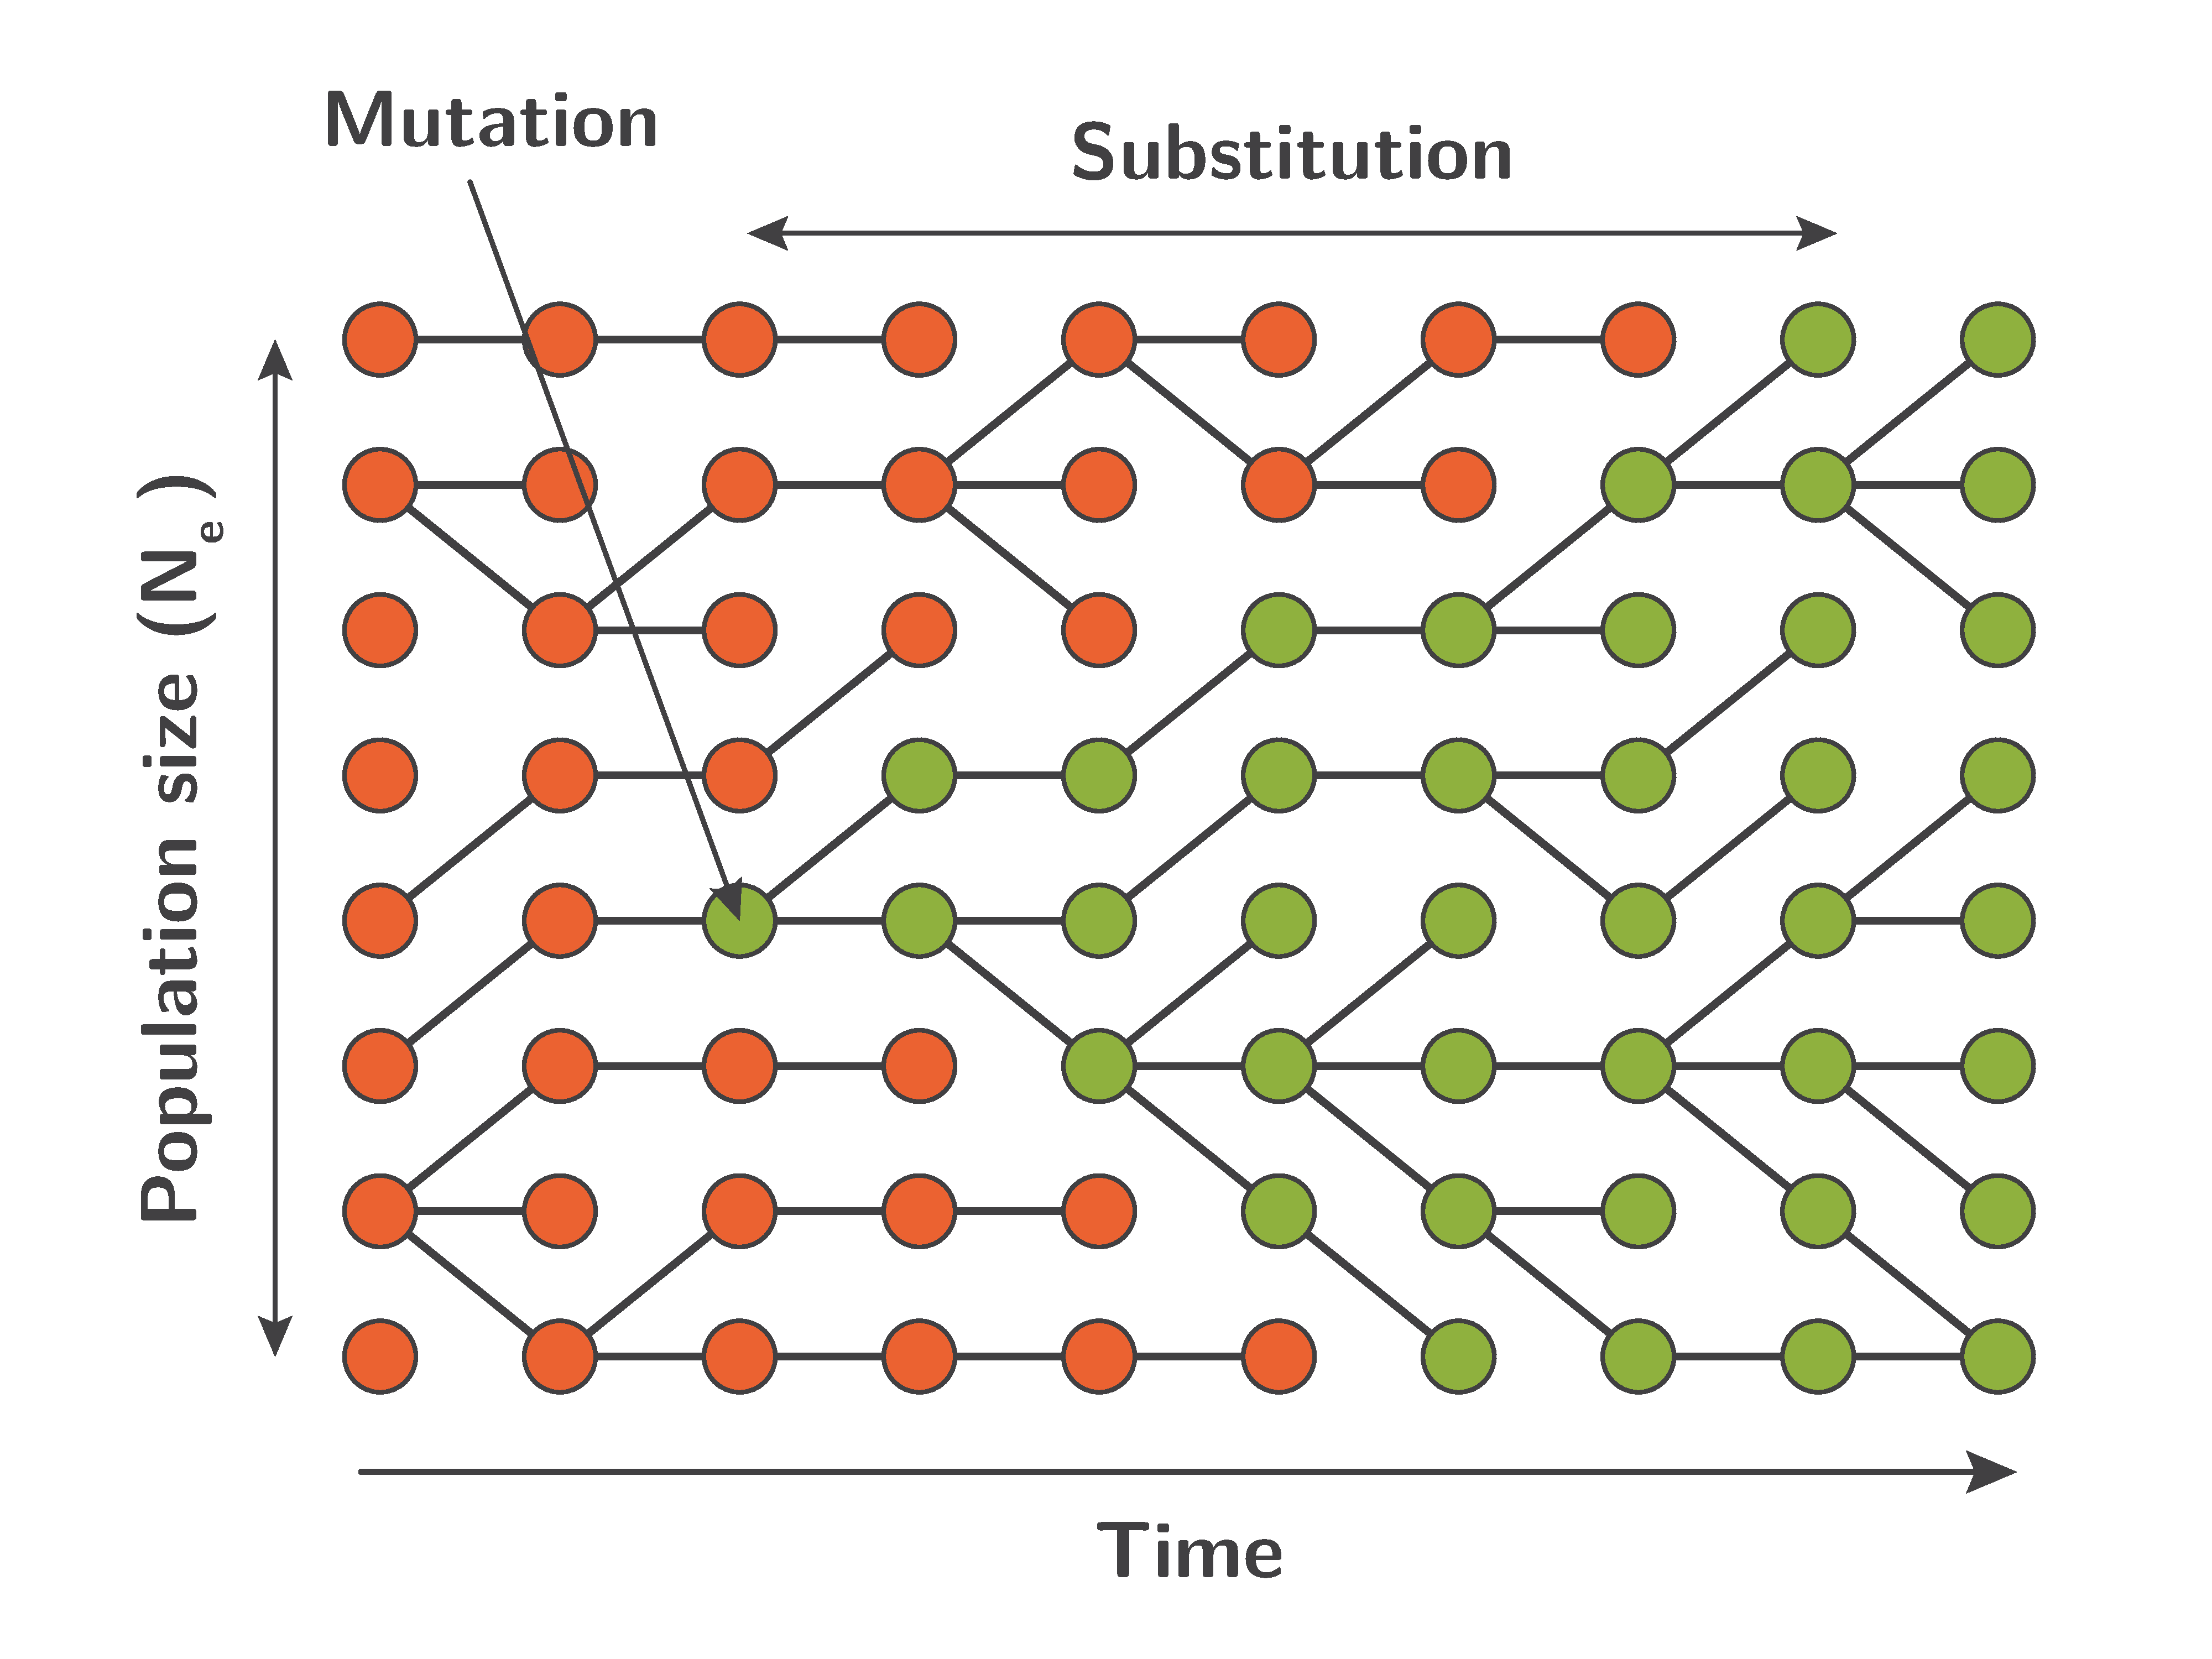
\includegraphics[width=0.6\textwidth]{figures/proba-fixation.pdf}
	\caption{Substitution rate}
\end{figure}
The mutation rate from codon $\ci$ to $\cj$ depends on the underlying nucleotide change between the codon, if $\ci$ to $\cj$ are only a mutation away, $\nucitoj$ denotes the nucleotide change between the codons. The codon mutation rate is then given by the mutation matrix ${\mutmatrix_{\nucitoj}}$. Altogether, the mutation rate from codon $\ci$ to $\cj$ is:
\begin{equation}
\begin{dcases}
\mu_{\itoj} & = 0 \text{ if } \cj \notin \Ni \\
\mu_{\itoj} & = \mu \mutmatrix_{\nucitoj} \text{ if } \cj \in \Ni
\end{dcases}
\end{equation}
In the case of synonymous mutations ($\cj \in \NiSyn $), the probability of fixation is independent of the original and target codon, and equal $1/2 \Ne$. Finally ${\submatrix_{\itoj}}$ simplifies to: 
\begin{align}
{\submatrix_{\itoj}} & { = 2 \Ne \mu_{\itoj}  p_{\mathrm{fix}}}(\itoj) \nonumber \\
{\submatrix_{\itoj}} & { = 2 \Ne \mu_{\itoj} \dfrac{1}{2\Ne}} \nonumber \\
{\submatrix_{\itoj}} & { =  \mu_{\itoj} } \nonumber \\
{\submatrix_{\itoj}} & { =  \mu \mutmatrix_{\nucitoj} }\text{, since } \NiSyn \subset \Ni \
\end{align}
In the case of non-synonymous mutations ($\cj \in \NiNonSyn $), the probability of fixation depends on the difference of fitness between the amino-acid encoded by the codons:
\begin{align}
{\submatrix_{\itoj}} & { = 2 \Ne \mu_{\itoj} p_{\mathrm{fix}}}(\itoj) \nonumber \\
& { = 2 \Ne \mu_{\itoj} }  \dfrac{2({\fitj - \fiti})}{{1 - \e^{4\Ne(\fiti - \fitj)} }} \nonumber \\
& { = \mu \mutmatrix_{\nucitoj} }  \dfrac{{\scaledfitj - \scaledfiti}}{{1 - \e^{\scaledfiti - \scaledfitj} }}\text{, where } \scaledfiti = 4\Ne \fiti
\end{align}
We can note that if the difference of fitness tends to $0$, the substitution rate equal the mutation rate:
\begin{align}
\lim_{\scaledfiti \to \scaledfitj} {\submatrix_{\itoj}} & { = \mu \mutmatrix_{\nucitoj} }  \dfrac{{\scaledfitj - \scaledfiti}}{{1 - (1  + (\scaledfiti - \scaledfitj)) }} \nonumber \\
& { =  \mu \mutmatrix_{\nucitoj} } 
\end{align}

\subsection{Steady state at equilibrium}
\citet{McCandlish2014}
We can calculate the steady-state solution of our model using the
analogy between evolutionary biology and statistical
physics recently demonstrated by Sella and Hirsh
(2005). The
key insight of Sella and Hirsh (2005) is that the prob-
ability pi to find the population in state i is proportional
to a function F(i) (also called a Boltzmann factor) that
depends only on the fitness of sequence i, the population size, and details of the mutation process.
where the sum runs over all possible sequences j.
Once we have the probabilities pi, we can calculate all observable quantities of interest, such as mean fitness and mean
evolutionary rate, using standard probability theory 

\subsection{Non-synonymous and synonymous substitution rate} 

The phylogeny-based method models the substitution rate at the codon level. Synonymous and non-synonymous mutations are treated differently. The rate of non-synonymous substitutions over the rate of synonymous substitutions (denoted $\omega=d_N/d_S$) is estimated as a parameter of the model \cite{Muse1994,Goldman1994}. Assuming synonymous mutations are neutral, an $\omega>1$ signals an excess in the rate of non-synonymous substitutions, indicating that the protein is under adaptive evolution. Conversely, a default of non-synonymous substitutions, leading to $\omega<1$, means the protein is under purifying selection. However, in practice, protein are typically under a mix of adaptation and purifying selection, thus typically leading to an $\omega<1$ even in the presence of positive selection. More sophisticated methods have been proposed. In particular, site-models trying to detect specific site of the sequence with an $\omega>1$, have been developed \cite{Yang2001, kosiol_patterns_2008}.
However these models potentially miss a substantial fraction of adaptation and do not quantify the rate of adaptation.  \\


\section{Mutation-selection analogy}
In this section, I'll develop reflections on apparent similarities and analogies between the mutation-selection process and other processes present in a variety of scientific fields, displaying the same underlying mechanism and emerging properties, though with different name and aspiration.
This effort is made in the aim of giving another view of the mutation-selection process, such as to better appreciate and conceptualize its assumptions, its limits, and the respective role of the different components. 
Such attempts requires to boil down the mutation-selection mechanism into its core components, while at the same time rephrasing the description using lexicography outside of population-genetic such as to open new perceiving angles.

At the bottom, mutation is a process creating diversity, changing and moving the current viable state to a novel and unknown position, fundamentally allowing exploration of the state space.
On the other hand, selection is the criteria on which a new state is deemed a disrupting innovation or a nonviable alteration, and allow to determine which changes to exploit and which to filter out and discard based on its fitness.
Fundamentally, reducing the diversity created by the mutation process is the very essence of selection.
Finally, drift arbitrate between the creation and reduction of the two processes, it dictates how much exploration of novelty is permitted, and conversely how much exploitation of only the fittest states is granted.

I argue that this creation and reduction process is found at the core of several research disciplines, while the link between them is scarcely made \citep{Baeck1994, Eiben1998}. 

\subsubsection{Metropolis-Hasting sampling}
Obtaining a sequence of random samples from a probability distribution can be difficult, especially when the number of dimensions is high.
However, the Metropolis-Hasting procedure based on a Monte Carlo Markov chain can sample from any probability distribution, provided that we know how to compute the probability density, or even less restrictively any function proportional to the density \citep{Hastings1970}.
This stochastic procedure which is based on three steps bears many similarities with the mutation-selection process:
\begin{itemize}
	\item Generate a stochastic candidate from the current state, analogous to the mutation.
	\item Calculate the acceptance ratio as the ratio of the two densities, analogous to the selection coefficient of the mutated state.
	\item Stochastic acceptance or rejection based on the acceptance ratio, a process analogous to drift. 
\end{itemize}
Inherently, is Metropolis-Hasting procedure is based on creating and subsequently reducing diversity, which allows to obtain a random sequence of samples from any distribution with a straightforward recipe, and is a critical tools in statistic and statistical physics.

\subsubsection{The exploration-exploitation dilemma}
Many mathematical, engineering and day-life problems are not about sampling a state space, but rather finding the optimal and best state given a criteria or a function to maximize.
Naturally, we would prefer deterministic (strictly reproducible) rather than stochastic optimizing strategies to be in searching the optimal state.
Unfortunately, whenever the state space is too large, often due to the curse of dimensionality, a greedy or heuristic search of an optimal state can performs atrociously \citep{Bellman1966}.
In high dimensional space, stochastic optimization tools have been deemed very valuable, such as stochastic gradient decent or so called evolutionary algorithm \citep{Russell2010,Vikhar2017}.
Inherently, they are based on two processes, one is stochastically creating diversity and exploring the state space, while the other is filtering the explored states and thus reducing the diversity.

In the constrained case of a finite number of time or attempts to find the best outcome overall, the problem is best described by the multi-armed bandit problem. The name comes from imagining a gambler at a row of slot machines (sometimes known as one-armed bandits), where each slot machine provides a random reward from a probability distribution specific to that machine. The player has to decide which machines to play, how many times to play each machine and in which order to play them, and whether to continue with the current machine or try a different machine, such as to maximize the sum of rewards earned through a sequence of lever pulls.
The gambler faces a dilemma at each trial, either reducing his regret by exploiting the best arm, or gain information by exploring other arms.
The best strategy to solved this dilemma can be mathematically derived in numerous cases, and encompass a mixing strategies with a defined ratio of exploration and exploitation \citep{Auer2002,Kocsis2006,Furnkranz2006}.
This problem is far from be only theoretical, and has be used to explain a multitude of phenomena, such as the movement of animals in novel landscapes, the most efficient resource allocation for a start-up company, the effects of old age on knowledge acquisition in humans, and in search of the most efficient treatment in clinical trials (hence the name a clinical arm) \citep{Berger-Tal2014, March}. 
An other application of the exploration-exploitation dilemma is AlphaGo, the first computational program mastering the board game go at the professional 9-dan level in 2017 and out-compete Ke Jie, the world n°1 ranked player at the time \citep{Silver2017, Silver2018}.
AlphaGo has often been publicized and hyped in various media outlets that this feat was possible due to machine learning, more specifically due to convolutionnal neural networks.
However, it is more scarcely mentioned that AlphaGo neural network is combined with an exploration-exploitation algorithm, or more specifically Monte Carlo tree search. 
In practice, the neural network is used as a criteria to measure the advantage of a board configuration, but the different moves and path probed and trimmed is done via an exploration-exploitation procedure. 
Of note, the convolutionnal neural networks use a stochastic gradient descend (mentioned above) to converges.

Altogether, exploration and exploitation, creation and reduction, mutation and selection, are different names that encompass the inherently same process efficiently sampling and optimizing whenever the state is too large to be traversed.
Of course, scientific research endeavor is also a exploration-exploitation dilemma, which is arguably externally pressured to pursue exploitation, trough funding of impactful research and a \textit{publish-or-perish} systemic culture in early career stage.

% As a side note, it appears that drift and selection are actually confounded, they are both on the side of exploitation, not on exploration.
As a side note, mutation is a necessary process of evolution, while sexe is not mandatory but increase the diversity of genomes between generations.
Arguably, studying evolution while disregarding mutation is a sufficient approximation whenever mutation rate and number of generations is low, which is developed thoroughly trough the whole field of quantitative genetics.
Sex and mutation are both generating new states and are part of the more general exploration facet.
This explains why sex is favored in fluctuating environments.

I argue that scientific fields studying and leveraging this pervasive process can gain knowledge with each others by interacting, much like there as been many crossover between economics and evolution.
Game theory had originally been developed to model economic actors behavior and strategies \citep{VonNeumann1947}, while latter being emerging as the framework of evolutionary dynamics, which explains the emergence of altruistic behaviours in Darwinian evolution, the conundrum of the existence of the peacock's tail and other such biological encumbrances \citep{Smith1973, Smith1982, Nowak2006}.
